\chapter{\label{ch:dev}Development practices}

As this is a new software project, we invested a significant effort in setting
up a development infrastructure to ensure our work is carefully tracked,
thoroughly and continually tested, and incrementally improved and documented.
To this end, we have adopted best practices for software development used by
successful open source projects \cite{millman2014}.

\section{\label{sec:vc}Version control}

We use Git\footnote{\url{http://git-scm.com}} as our version control
system (VCS) and GitHub\footnote{\url{https://github.com}} as the public hosting
service for our official \texttt{upstream} repository.  Git allows us to
carefully track how our code evolves as well as deliberately consider and
refine new functionality on isolated branches before merging it into the main
branch.

\subsection{Git data model}

Git's data model is sufficiently different from other VCS that it is helpful to
briefly describe it before discussing our Git workflow.  In Git, a repository
is represented as a directed acyclic graph (DAG) of commits.  A commit in Git
is a cryptographically signed object containing zero or more parent commits,
some metadata, and a snapshot of entire work tree.  A working tree can be
thought of as the entire project structure of directories and files at a
particular point in the development.  Over time the working tree evolves due to
new features, refactoring of current functionality, optimizations, or bug
fixes.  Taking snapshots of this evolution over time allows us to analyze the
past to better understand how the code came to be in its present state.  The
cryptographic signature ensures that it is practically impossible for someone
to change history without it being readily apparent.\footnote{Surprisingly
few previous VCS even attempted to ensure the historical integrity of a
project's history.}

An essential design feature of Git (and one absent from other VCS), is
the simplicity of creating and merging branches.  A branch in Git is a pointer
to a commit in the repository DAG, which moves forward as new commits are made.
This provides a lightweight mechanism for branching.  Typically each repository
has a master branch which is viewed as the main truck of development.  Creating
a new branch off the master branch (or main trunk) only requires making a new
label and then committing to it.  A merge is a commit with 2 or more parents,
which corresponds to the resulting integration of the parent commits.

Further, Git is completely decentralized so there are no inherent
asymmetries as found in older client-server models.  So every developer
has their our own self-contained repository.  For collaborative purposes,
Git repositories have a notion of remote repositories.  Remotes are other
repositories that a specific repository tracks.  Commits can be pushed
and pulled from remote repositories into local repositories.

Git, while not easy to master, is simple in the sense that once a few concepts
are understood, it behaves in an entirely reliable, intelligible, and
straightforward manner.\footnote{To clarify the distinction I am making between
easy and simple, let me use the familiar example of Calculus.  Many students
require one or more semesters of college level coursework to learn the basic
techniques of differentiation and integration.  In this sense, it isn't easy to
learn.  However, once the basic techniques are learned, it is simple to apply
to new contexts and applications.  Prior to the invention of Calculus,
discovering how to compute the area under a new curve often required
mathematical genius and insight into the specific application.} If you've ever
tried to do anything non-trivial in ``easier'' to use VCS such as SVN or CVS,
then you've likely experienced the ensuing frustration these systems cause.
More likely you've never tried to do anything non-trivial with such systems as
it is completely unclear how such things could be done.  With Git the pain is
upfront, but the benefits are extensive and enable fluid and comprehensive
collaborations, which scale well.

The inherent flexibility of Git makes numerous workflows possible.  We've
followed the standard workflow used by the core scientific Python packages.
This workflow enables us to keep the official master branch of the project in a
pristine state at all times and simplifies the structure of the DAG by
divorcing it from the sometimes random, tentative moves made when developing
new code so that we can record a revised and coherent history.  Further it
rationalizes the process of making changes to the official master by allowing
us to add new features and bug fixes in isolated, tested, and code reviewed
chunks.

We've designated \url{https://github.com/statlab/permute} as the official
upstream master.  No one commits changes to it directly.  Instead we each fork
this repository on GitHub (e.g, my fork is
\url{https://github.com/jarrodmillman/permute}).  To fork a project on GitHub,
you click a button labeled fork on the repository website you wish to fork.
This let's GitHub track the relationship between various repositories it hosts.
In particular, it enables you to create pull requests, which I discuss below.

Once we've forked the official repository, we clone our fork onto a local
account so we can work on the code.  Rather than work on the \texttt{master}
branch of our repositories, we perform all code changes on branches.  As
we work on our branch we push the changes to our individual forks.  Once
we've pushed our branch to our fork on GitHub, we can create a pull request
to begin the code review process necessary to merge our branch into the
upstream master.

To get new code integrated in the official \texttt{upstream} master, we use
GitHub's \emph{pull request} mechanism.  This helps make performing code review
for new code added to the official ``upstream'' repository easy to manage.
Given the short development history and small development team, we have
kept the review process lightweight and mostly automated, which I describe
below.

Once a \emph{pull request} is reviewed and accepted, it is merged into
the upstream master.  Once merged into the upstream repository, we pull
the changes into our local repository and then cleanup after ourselves.

To summarize, all new work is made on a branch and pushed to our
personal forks of the upstream repository. To incorporate this new
work on our local master branch we then pull from the upstream
master.  This separation between where we push and pull our
work creates the space for code review, testing, and discussion of
new features and bugfixes before merging work into the official 
repository.

\section{\label{sec:test}Testing}

We use the \texttt{nose} testing framework for automating our testing
procedures.\footnote{\url{https://nose.readthedocs.org}}  This is the standard
testing framework used by the core packages in the scientific Python ecosystem.
Automating the tests allows us to monitor a proxy for code correctness when
making changes as well as simplifying the code review process for new code. 

The \texttt{nose} testing framework simplifies test creation, discovery,
and running. It has an extensive set of plugins to add functionality
for coverage reporting, test annotation, profiling, isolation, as well
as inspecting and testing documentation.

So far, we've primarily used it for testing individual units of code for
consistency.  Eventually we will add regression and integration testing as well
as testing the code for correctness using the expected statistical properties.
For instance, rather than merely checking whether when a function is called
with the same arguments it returns the same results, we can run tests that
check whether results are within the expected statistical error.

%While testing is not a proof of program correctness, it can serve as a
%useful tool for catching errors and increase our confidence in the
%reliability of our results.

%For example, from the top-level of the repository, you can ask \texttt{nose}
%to run the tests by entering \texttt{nosetests permute} in Bash.  For example,
%
%\begin{verbatim}
%$ nosetests permute
%.......................................
%----------------------------------------------------------------------
%Ran 39 tests in 48.957s
%\end{verbatim}
%
%In the above console output, you will see a ``.'' for each test, which
%is run.  A test corresponds to a function and each test may test several
%things.

%\subsection{Coverage}

We also use \texttt{nose} to monitor our test coverage.  Our goal is to
test every line of code.  For example, not only do we want to test every
function in our package, but if a specific function has internal logic
we want to test each possible path through the function.  Having tested
each line of code increases our confidence in our codebase, but more
importantly provides us assurance that changes we make do not break
existing code.  It also increases our confidence that new code works,
which reduces the friction of accepting contributions.

%Working in the top-level of our local repository in Bash, you could
%enter
%
%\begin{verbatim}
%$ nosetests permute --with-coverage --cover-package=permute
%.......................................
%Name                 Stmts   Miss Branch BrMiss  Cover   Missing
%----------------------------------------------------------------
%permute                 43      5     10      1    89%   77-88
%permute.core            60      0     30      4    96%   
%permute.data            45      0      2      0   100%   
%permute.eda             22      0      8      0   100%   
%permute.irr             52      0     20      1    99%   
%permute.stratified      45      0     16      1    98%   
%permute.utils           10      0      6      0   100%   
%----------------------------------------------------------------
%TOTAL                  277      5     92      7    97%   
%----------------------------------------------------------------------
%Ran 39 tests in 56.023s
%
%OK
%\end{verbatim}
%Here you can see, that in addition to running 39 tests without error,

Currently over 97\% of our code has at least one test touch it.  The remaining
lines are mostly branch misses where executing both branches is difficult.  For
example, the branch depends on the particular environment in which it is being
run. So each branch is tested in different environments, but not at the same
time.  I've tried to trick the tests to run both branches by hand modifying
system objects in the tests as well as creating mock objects, but haven't been
able to achieve 100\% coverage.

%\subsection{Continuous integration}

Having an automated test suite enables us to implement continuous integration.
Continuous integration is the process of automatically running the full test
suite using different versions of our dependencies (e.g., Python 2 and 3) on
different operating systems (e.g., Windows, Mac OS, and Linux) and different
hardware (e.g., Big-endian and Little-endian systems) every time any new commit
is made to a repository or pull request.

We've configured Travis CI\footnote{\url{https://travis-ci.org}} and
\texttt{coveralls}\footnote{\url{https://coveralls.io}} to be automatically
triggered whenever a commit is made to a pull request or the upstream
master directly.  These systems run the full test suite and generate reports.
These systems are integrated with GitHub so that our pull requests are
automatically annotated with these reports as soon as changes are made.

%Python 2 and Python 3 on Debian-derived system
%
%I run the tests for both Python 2 and Python 3 on a RedHat-derived system
%
%While Philip and Kellie run the tests for Python 2 on Mac OS.
%
%need to add additional build systems to buildbot nipy.bic.berkeley.edu...
%
%\texttt{coveralls}\footnote{\url{https://coveralls.io}}
%
%\begin{figure}
%  \begin{centering}
%    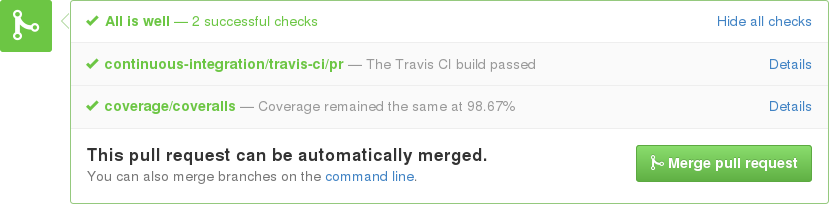
\includegraphics[width=5.5in]{fig/pull-request-ci.png}\par
%  \end{centering}
%
%  \caption{\label{fig:pull-request}Pull request and continuous integration.}
%\end{figure}

\section{\label{sec:doc}Documentation}

Reducing the
friction involved with producing documentation encourages developers and users
to contribute documentation.  For instance, NumPy use to have fairly poor
documentation until one summer when Stefan van der Walt (now a BIDS fellow)
built on several newly improved Python technologies for documentation
\cite{SciPyProceedings_27}.

We've adopted this system and already have good developer documentation and the
foundation for high-quality user documentation. We've used Python docstrings and
the NumPy docstring standard to document all the modules and functions in
\texttt{permute}.\footnote{https://github.com/numpy/numpy/blob/master/doc/HOWTO\_DOCUMENT.rst.txt}

Using Sphinx and some NumPy extensions, we have a system for autogenerating the
project documentation (as HTML or PDF) using the docstrings as well as
stand-alone text written in a light-weight markdown-like language.  This
enables us to embedded references, figures, code that is auto-run during
documentation generation, as well as mathematics using \LaTeX.

\section{\label{sec:release}Release management}

Our development workflow ensures that the official upstream master is always
pristine and ready for use.  This means anyone can get our official upstream
master at any point, install it and start using it.  However, it is still
desirable to periodically make official releases with binary packages uploaded
to PyPI (the Python version of CRAN) and release announcements posted to
community lists.

Since the project is still new, there's only been one release so far.  To install
this release without downloading the source code, you can enter the following
command from a Bash prompt:
\begin{verbatim}
pip install permute
\end{verbatim}
This will install version 0.1.alpha0 of \texttt{permute} as well as it
dependencies.  Since we have yet to finalize our call signatures or package
structure, we use the alpha designation to telegraph this fact to
potential users.  However, our release process is fully documented and
partially automated.  Together with the policy of keeping upstream master
pristine, this means that making new releases is extremely light-weight.  Being
able to quickly generate new releases quickly and reliably is essential to being able to
quickly respond to mistakenly broken releases.  Despite using a rigorous
testing and integration methodology, error is a constant concern.  Being able
to quickly respond to discovered errors in released software is essential to
creating a software tool people trust.
